\documentclass{article}
\usepackage{comment}
\usepackage[final]{styles}
\usepackage[utf8]{inputenc} % allow utf-8 input
\usepackage[T1]{fontenc}    % use 8-bit T1 fonts
\PassOptionsToPackage{hyphens}{url}\usepackage{hyperref}       % hyperlinks
\usepackage{url}            % simple URL typesetting
\usepackage{booktabs}       % professional-quality tables
\usepackage{amsfonts}       % blackboard math symbols
\usepackage{nicefrac}       % compact symbols for 1/2, etc.
\usepackage{microtype}      % microtypography
\usepackage{amsmath}
\usepackage{amsthm}
\usepackage{amssymb}
\usepackage{tikz}
\usepackage{csquotes}
\usepackage{float}
\usepackage{graphicx}
\usepackage{wrapfig}
\usepackage{multicol}

% \title{Harmonic Flows on Guage Equivariant Moduli Space of Connection }
% \title{Ergodic Flows on Guage Equivariant \\ Space of Connection }
% \title{Ergodic flow on Moduli\\  Space of Connections }
% \title{Attention and Energy Minimization \\ on Moduli  Space of Connections }
\title{Energy Minimizing Flows on \\ Equivariant Space of Connections }
% \title{Learning Energy Minimization on \\  Moduli Space of Connections }

% The \author macro works with any number of authors. There are two commands
% used to separate the names and addresses of multiple authors: \And and \AND.
%
% Using \And between authors leaves it to LaTeX to determine where to break the
% lines. Using \AND forces a line break at that point. So, if LaTeX puts 3 of 4
% authors names on the first line, and the last on the second line, try using
% \AND instead of \And before the third author name.

\author{%
  L. J. Pereira \\
%   \texttt{lukejoepereira@gmail.com} \\
  % examples of more authors
  % \And
  % Coauthor \\
  % Affiliation \\ consciousness
  % Address \\
  % \texttt{email} \\
  % \AND
  % Coauthor \\
  % Affiliation \\
  % Address \\
  % \texttt{email} \\
  % \And
  % Coauthor \\
  % Affiliation \\
  % Address \\
  % \texttt{email} \\
  % \And
  % Coauthor \\
  % Affiliation \\
  % Address \\
  % \texttt{email} \\
}

\begin{document}
\setlength{\abovedisplayskip}{4pt}
\setlength{\belowdisplayskip}{4pt}

\vspace{-2cm}
\maketitle


\vspace{-1.3cm}

\begin{comment}
\begin{abstract}

% A novel energy-based learning model is described using gauge theory and is speculated to produce dynamics similar to those in found in neuronal activity. 
In gauge theory, the moduli space of connections results from quotienting the space of principal connections of a fiber or vector bundle by the structure group, generating a gauge equivariant space. A moduli space of connections can be used to cover the activity of a collection of deep neural networks, which are represented as trajectories on vector bundles. On this upper bounding space, a top-down energy-based attention mechanism can be trained from activity of the bottom-up trajectories of the underlying networks through a composition of energies. Dynamics of attention are computed by minimizing the energy functional of the space; in particular, the Yang-Mills moduli space, a subset of the total connection space, can be constructed to be a smooth, compact, and oriented manifold in 4 dimensions with critical points known as Yang-Mills connections (or instantons). 
% The harmonic model can be applied to these dynamics with behaviour comparable to connectome-specific self-localized critical waves. 
Examining mathematical research in ergodic and hyperbolic dynamics of moduli spaces allows the ergodic free-energy minimizing model described in previous works to be developed further.
An autoencoding method using the cobordism property of the space is considered.

% This yang mills space of connection curvature can be represented with holomorphic vector bundles on which variational noise generates energy-based attention. In a statistical learning and information geometry setting, this space can be viewed as a kernel manifold which interfaces with specialist neural networks in a product of experts summation. This formulation of general intelligence provides a simple and biologically plausible model of 
 

% Fiber bundles of manifolds from differential geometry can be applied to the meta-learning task of the classification of subtasks to subnetworks. Assuming the input of a typical machine learning task can be associated with some Lie Group, then a differentiable manfiold can be constructed to represent the space of all tasks. Using gauge theory, this manifold can be  formalized as a Yang-mills moduli space.
\end{abstract}

\end{comment}

% gauge Dynamics of moduli spaces
\section{Overview}
In gauge theory, the moduli space of connections results from quotienting the space of principal connections of a fiber or vector bundle by the structure group, generating a gauge equivariant parameter space. A moduli space of connections can be used to cover the activity of a collection of hierarchical or deep neural networks, represented as trajectories on vector bundles. On this upper bounding space, a top-down energy-based attention mechanism can be trained from sampled activity of the bottom-up trajectories of underlying networks through a composition of energies. Dynamics of attention are computed by minimizing the energy functional of the connection space. In particular, the Yang-Mills moduli space, a subset of the total connection space, can be constructed to be a smooth, compact, and oriented manifold in 4 dimensions with critical points known as Yang-Mills connections (or instantons). These connections minimize curvature between bundles and, from an information geometric perspective, they minimize relative entropy or KL divergence between two gauge equivariant manifolds. Allowing these connections to function as sources of variational noise, we train a neural network to minimize total energy of the moduli space. This process can be understood as finding stable solutions of an intrinsic flow on the curvature metric, producing a Ricci Yang-Mills flow with solutions akin to Ricci solitons. Stable solutions represent islands of agreement formed through consensus within a dynamic part-whole hierarchy. The theoretical objects representing solutions of these flows are studied as quasiparticles and can be made physical in quantum materials or gasses. Our geometric formulation of general intelligence provides a natural and biologically plausible model for quantum AI. 
% Moreover, fusing physical field theories with neuroscience and ML may justify introspection into the Anthropic Principle and cosmological fine-tuning. 

% Exploratory musings in quantum machine learning describe a quasiparticle in a bose-enstein condesate of the Yang-mills moduli space described earlier. To do so, a control system must train the condesate using boltzman machines to allow the quasiparticle to endure. This quasiparticle represents the state of the Moduli space of connections  after a Wick rotation of the 4-dimensional space into bosons in 3-dimensional space.
% by minimizing the relative entropy or KL divergence between active bundles.
% The harmonic model can be applied to these dynamics with behaviour comparable to connectome-specific self-localized critical waves. 


\section{Geometry of Latent Information}
\subsection{Manifolds, Vector bundles, Connections}
    A fiber bundle serves as a useful mathematical object to analyse both the recursive construction of artificial and biological neurons and neural networks, as well as providing fitting descriptions of the geometry of latent information, which uses manifold representations for information processing and statistical learning.
    % Finer details can be found in my notebooks on differential geometry, Lie groups and algebras, and gauge theory.
    A fiber bundle formalizes the notion of one topological space (called a fiber) being parameterized by another topological space (called a base). The bundle comes with a group action on the fiber that represents different ways the fibers can be viewed as equivalent. Bundles also have a property, known as local trivialization, allowing neighborhoods of the bundle to be computed as simple, oriented product spaces, despite the global space  being unoriented or twisted.
    
    A family of fibers associated to a base can be described by defining a standard (or template) fiber which all other fibers are isomporphic to. This is formalized by defining a diffeomorphic or homotopic projection mapping, that connects positional data from the entirety of the space of fibers to a base, and implicitly from one fiber to another. When the template fiber is a vector space, the bundle is called a vector bundle. Similarly, a standard connections between fibers exists, known as a principal Ehresmann connection, and can be understood as a covariant directional derivative on the tangent spaces of the manifolds. Intuitively understood, Lie groups have a special recursive nature as a result of the group being itself a differentiable manifold. An interesting phenomena occurs when equipping a bundle with a Lie group action; the bundle structure can be used to represent both the original vector bundle as well as a higher-level collection of mappings of their tangent spaces, in what's known as a bundle of connections. 
    % To be expanded in the section on moduli spaces, the Yang-Mills or instanton connections within this bundle of connections correspond to those that minimize their curvature. 
    
% \newpage
    

\subsection{A Priori Structure Groups}
    
    % Hebbian learning is a form of activity-dependent synaptic plasticity where correlated activation of pre- and postsynaptic neurons leads to the strengthening of the connection between the two neurons. Another central theory of cognitive neuroscience is that different parts or modules of the brain perform different functions, known as functional localization.
    % We can develop a simple partition scheme by initially assigning a Bernoulli random variable to each synapse. Then, while ``zooming out" we merge random variables together based on their covariance and locality to build a course-grained model. Recall, \textit{covariance} is a measure of the joint variability of two random variables and is increasingly positive when the variables tend to show similar behavior and grow increasingly negative when dissimilar. This conversion of physical synapses into a set of random variables can be described with Markov partitions and Bernoulli Schemes. 
    % At each step, the accuracy of the model naturally decrease as a result of merging imperfectly covariant random variables.
    %     However, some form of a priori covariance is necessary for maintaining information integrity through bilateral and hierarchical dynamics, i.e. to allow a connection to communicate in a general and equivariant way between modules and within their intrinsic substructures. 
    
    % \begin{wrapfigure}{r}{0.5\textwidth}
    %     \begin{center}
    %     \includegraphics[width=0.43\textwidth]{DTI-sagittal-fibers.jpg}
    %     % \caption{Fiber tracts that run through the mid-sagittal plane}
    %     \end{center}
    % \end{wrapfigure}
    
   A biological first principle of covariance arises naturally from analysis of neuronal activity, which favours functional localization and Hebbian learning.
    Moreover, cognitive networks in the brain flow in connectome-specific diffusive waves along gyrification paths, which are theorized to be caused by differential tangential growth. 
    Recall, covariance is a measure of the joint variability of a pair random variables (or synapses) and is increasingly positive when the pair show similar behavior and is negative when dissimilar.
    Moving from discrete random variables to fields and continuous manifolds (like EM fields), the covariant derivative between fibers of a bundle naturally arises and is known as a principal Ehressmann connection. To allow holonomy of dynamics on a bundle, it is necessary to impose a generalized a priori covariance principle to maintain integrity of information during parallel transportion in bilateral and hierarchical directions.
    Yet for a standard learning model, covariance of functionality is an a posteriori feature since the joint variability is unknown until individual modules are fully trained. 
    Covariance of fibers can be achieved by imposing the structure group to be a Lie Group, but can also be achieved by imposing restrictions on the projection map of Riemannian manifolds without explicitly defining the structure group beforehand (Gao, 2021).
    
    % \begin{figure}[h]
    %     \centering
    %     \includegraphics[width=5.5cm]{DTI-sagittal-fibers.jpg}
    %     \caption{Fiber tracts that run through the mid-sagittal plane}
    % \end{figure}
    
    % \begin{figure}[h]
    %     \centering
    %     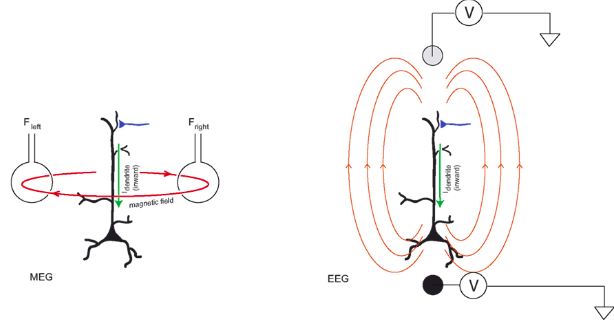
\includegraphics[width=8cm]{eeg-meg-neuron.png}
    %     \caption{Diffusive electric and magnetic signals in neurons}
    % \end{figure}

    
    
\subsection{Moduli Spaces}
    With covariance established on connections, it becomes possible to perform inference using higher levels of abstraction on gauge fields. This is done by constructing a gauge equivariant bundle of connections known as a moduli space of connections, which can be further reduced to a Yang-Mills moduli space defined to be a finite dimensional manifold. This reduced space has local and global minima being connections with minimized energy known as Yang-Mills connections or instantons. Yang-Mills connections serve as a natural choice of connection on principal and vector bundles since they minimize their curvature. From an information geometric perspective, this can be thought of as minimizing relative entropy between sampled trajectories of two manifolds which happen to be gauge equivariant. The gauge field strength is the curvature $F_{A}$ of the connection, and the energy of the gauge field is given by the Yang–Mills action functional:
    \begin{equation}
         {\displaystyle \operatorname {YM} (A)=\int _{X}\|F_{A}\|^{2}\,d\mathrm {vol} _{g}.}
    \end{equation}
    With the aim of having zero or vanishing curvature, we vary paramaters in search of a connection with curvature as small as possible. The Yang–Mills action functional simply corresponds to the $L^{2}$-norm of the curvature, and its Euler–Lagrange equations describe the critical points of this functional, either the absolute minima or local minima.   

% \vspace{-0.3cm}
\section{Variational Geometric Flows}
\subsection{Variational Inference and Energy Composition}
    As underlying neural networks perform inference, their latent vector trajectories pass through hierarchies of weighted hidden layers in a bottom-up manner. At the same time, a top-down variational noise is produced around the instanton solutions that best minimize energy of the total activity on the moduli space of connections. Using an energy-based model (EBM) we sample the joint distribution as a sum of each latent trajectory, corresponding to a product of experts model. This forms an attention mechanism that is learned on the top-down manifold as well as creating a generative effect on underlying networks through variational inference. The idea behind variational methods is to pick a family of distributions over the latent variables with its own variational parameters, $q(z_{1:m} | v)$, and then attempt to find the setting of the parameters that makes $q$ close to the posterior of interest (the instanton). Closeness of the two distributions in variational inference is measured with the Kullback-Leibler (KL) divergence, 
    \begin{equation}
         \displaystyle KL(q||p)=  E_q\bigg[ \log \frac{ q(z)}{p(z | x)} \bigg].
    \end{equation}
    % $ \ \ \displaystyle KL(q||p)=  E_q\bigg[ \log \frac{ q(z)}{p(z | x)} \bigg].
    % $
    \begin{figure}[H]
        \centering
        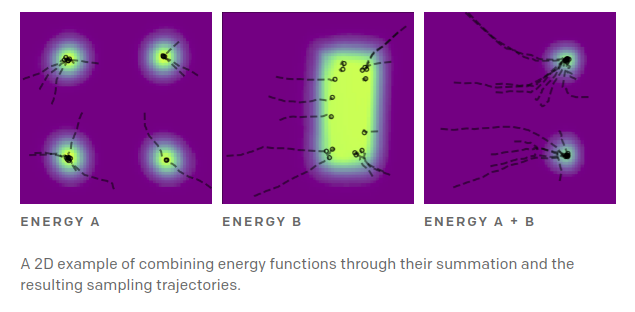
\includegraphics[width=13cm]{openai-ebm.png}
        \vspace{-0.87cm}
        \\  (Yilun, 2019)
        % \caption{Fiber tracts that run through the mid-sagittal plane}
    \end{figure}
    
\subsection{Geometric Flows}
    
    \begin{wrapfigure}{r}{0.4\textwidth}
        \vspace{-0cm}
        \centering
        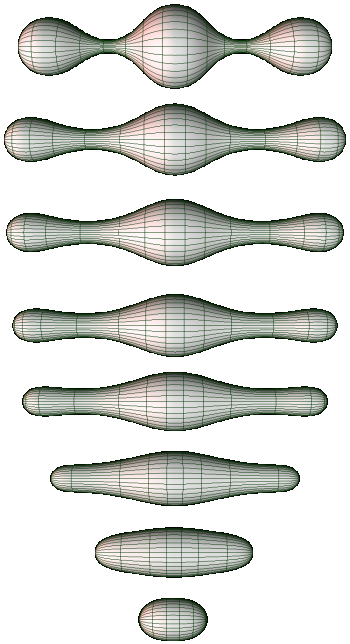
\includegraphics[scale=0.3]{ricci-flow.png}
        % \caption{Ricci flow visualization (Rubinstein, 2005)}
        \\ Ricci flow of a metric manifold (Rubinstein, 2005)
    \end{wrapfigure}
    
    We can interpret energy minimization through variational methods as a geometric flow on the moduli space (for intrinsic flows) or on the parameter space (for extrinsic flows). A Ricci flow is an example of an intrinsic flow on the metric, whereas a mean curvature flow (as found in soap films, with critical points as minimal surfaces) is an example of an extrinsic flow on an embedded manifold. The variational method for minimizing energy described previously can be understood as a mix of the two; changing both the embedded manifolds constructed with hierarchical neural networks and the moduli space of connections (or metric) itself. We can further classify it as both a variational and curvature flow since it evolves to minimize the Yang-mills action functional which is the $L^2$ norm of curvatures. The Ricci flow, Calabi flow, and Yamabe flow all arise in similar ways. Curvature flows may not necessarily preserve volume (the Calabi flow does, while the Ricci flow does not), meaning the flow may simply shrink or grow the manifold, rather than regularizing the metric. To avoid this, it's possible to normalize the flow by fixing the volume.

    \subsection{Islands in Part-Whole Hierarchies}
    The GLOM model (Hinton 2021) aims to represent part-whole hierarchies, using islands of matching vectors, known as islands of agreement, to construct nodes in parse tree representations within a neural network. A part-whole hierachy is simply a system consisting of subsystems or components that can themselves be broken down into further subcomponents. By finding clusters of coherence, the model attempts learn intuition and analogical reasoning by encoding parts that are not well defined, unconscious, or possibly obscured. Moreover, Hinton describes the importance of  viewpoint and coordinate-invariance allowing for exchangibility within the network, which can be used to adapt to and generate novelty in a way similar to humans. We can draw comparisons between the GLOM model and learning energy minimizations on a moduli space, where vector encodings correspond to trajectories on vector bundles, frame invariance corresponds to the gauge invariance established by quotienting the space of principal connections of the vector bundles by Lie structure groups, and islands of agreement correspond to using variational, curvature Geometric flows that manifest stable instanton or soliton solutions. 
    
    Iterative consensus generally doesn't converge in coherent ways because of the difficulty of encoding a prior understanding of desirable representations to be generated through the agglomerative clustering. However, using a geometric model we find that we are better posed to converge to coherent clusters because of the use of an a priori structure groups which imposes meaningful symmetry to the clusters and an optmized organization of information throughout the space. Moreover, using Ricci flows to interpret the process, we gain access to a trove of mathematical research on the solubility, stability, and other convergence properties and behaviour.
    
\subsection{Variational Methods in EBMs}
    An energy function $E$ in an EBM can be thought of as an unnormalized negative log probability. 
    To convert an energy function to its equivalent probabilistic representation after normalization,
    % Recall, marginalisation is a method that sums over the possible values of one variable to determine the marginal contribution of another. 
    $P(y \mid x)$, we apply the Gibbs-Boltzmann formula with latent variables $z$ being marginalized implicitly through integration, i.e. $P(y \mid x) = \int_z P(y,z | x)$. Then,
    \begin{align*}
        P(y \mid x) &= \frac{ \int_z \exp(-\beta E(x,y,z)) }{ \int_y \int_z \exp(-\beta E(x, y, z))} 
    \end{align*}
    The derivation introduces a $\beta$ term which is the inverse of temperature $T$, so as $\beta \rightarrow \infty$ the temperature goes to zero, and we see that $\check{y} = \text{argmin}_{y} E(x,y)$. This inverse temperature limit appears similar to the critical temperature in BEC. We can redefine our energy function as an equivalent function with free energy $F_\beta$,
    \begin{align*}
        F_{\infty} (x,y) &= \text{argmin}_z E(x,y,z)\\
        F_{\beta} (x,y) &= -\frac{1}{\beta} \log \int_z \exp(-\beta E(x,y,z)).
    \end{align*}
    If we have a latent variable model and want to eliminate the latent variable $z$ in a probabilistically correct way, we just need to redefine the energy function in terms of $F_\beta$,
    \begin{equation}
         P(y \mid x) = \frac{ \exp(-\beta F_\beta(x,y,z)) }{ \int_y \exp(-\beta F_\beta(x, y, z))}.
    \end{equation}
    With variational methods, instead of only minimizing the energy function with respect to $z$ we must prevent the energy function from being 0 everywhere by constraining the flexibility of the latent variable $z$. The energy function is defined as sampling $z$ randomly according to a distribution whose logarithm is the cost that links it to $z$. This distribution is commonly chosen to be a Gaussian with mean $\bar z$ which results in Gaussian noise being added to $\bar z$. The reparameterization trick is often used to allow for backpropagation during training despite the random sampling.

    
    \section{Topological Quantum Computing (Exploratory)}

     % \subsection{Solitons and Instantons}
    \subsection{Quasiparticles}
    
    % \begin{comment}
    % quasiparticles and collective excitations
    % - Instantons and solitons
    
    % - Ricci solitons
    % https://math.stackexchange.com/questions/802933/ricci-soliton-geometric-meaning
    
    % - RICCI YANG-MILLS SOLITONS
    % https://arxiv.org/pdf/0907.1095.pdf
    % https://arxiv.org/pdf/2102.09538.pdf
    
    % \end{comment}
    
    Quasiparticles and collective excitations are emergent phenomena that encapsulate sections of a microscopically complicated system with their behaviour imitating different behaviour of weakly interacting particles in a vacuum. 
    A soliton is a localized, non-dispersive solution of a nonlinear theory in Euclidean space and is a real object. Conversely, instantons are not real and only exist as solutions to the equations of motion of a quantum field theory after a Wick rotation, in which time is made imaginary. Note, a Wick rotation is a transformation that substitutes an imaginary-number variable for a real-number variable in order to solve a problem of (complex) Minkowski space in Euclidean space. Therefore, instantons are not observable, but are used to calculate and explain quantum mechanical effects that can be observed, such as tunneling. In quantum chromodynamics (QCD), instantons are believed to tunnel between the topologically different color vacua.
    
    Given a smooth manifold $M$ and an open real interval $(a,b)$, a Ricci flow assigns to each $t\in (a,b)$ a Riemannian metric $g_t$ on $M$ such that
    \begin{equation}
        {\displaystyle {\frac {\partial }{\partial t}}g_{t}=-2\operatorname {Ric} ^{g_{t}}.}
    \end{equation}
    
    Ricci solitons are exactly the solutions to the Ricci flow that are of the form
    \begin{equation}
        g(t)=\sigma(t)\phi^{*}_tg_0
    \end{equation}
    where $g_0$ is some fixed metric, $\phi_t$ is a one-parameter family of diffeomorphisms with $\phi_0=id$, and $\sigma$ is a real-valued function satisfying $\sigma(0)=1$ (so that $g(0)=g_0$). One can picture the Ricci flow in this situation as moving the manifold around by internal symmetries (the family of diffeomorphisms) and a uniform-in-space scaling at each time. In this sense, the intuition is that the manifold maintains the same shape but expands or contracts. In the standard quantum field theoretic interpretation of the Ricci flow in terms of the renormalization group, the parameter $t$ corresponds to length or energy rather than time

    Aside from providing a quantum computational schema, it's also worth noting the philosophical implications of associating mathematics of physical unified field theories with neuroscience and machine learning theory. Namely, that it  may justify further introspection into the Anthropic Principle and the nature of cosmological fine-tuning which appears to be reflective in our own consciousness.

    
    \subsection{Bose-Einstein Condesate}
    
    % In quantum mechanics, variational method are used to find approximations of the lowest energy eigenstate or ground state, and some excited states which allows for calculating approximate wavefunctions. Variational methods can also be used to calculate position and trajectories of instantons. 
    
    A Bose–Einstein condensate (BEC) is a state of matter which is typically formed when a gas of bosons at low densities is cooled to temperatures very close to absolute zero causing a large fraction of the bosons to occupy the lowest quantum state, at which point microscopic quantum mechanical phenomena, particularly wavefunction interference, become macroscopic. This transition to BEC occurs below a critical temperature that is given by:
    \begin{multicols}{2}
    \noindent
    \begin{align*}
        \\
        \\
        \displaystyle T_{\rm {c}} &=\left({\frac {n}{\zeta (3/2)}}\right)^{2/3}{\frac {2\pi \hbar ^{2}}{mk_{\rm {B}}}} 
    \end{align*}
    \begin{align*}
        {\displaystyle \,T_{\rm {c}}} \,  &\text{is the critical temperature,}\\
        \displaystyle \,n \, 	 &\text{ the particle density,}\\
        {\displaystyle \,m}	\, &\text{the mass per boson,}\\
        {\displaystyle \hbar } \, 	&\text{the reduced Planck constant,}\\
        {\displaystyle \,k_{\rm {B}}}\, 	&\text{the Boltzmann constant and}\\
        {\displaystyle \,\zeta }\, 	&\text{the Riemann zeta function;}
    \end{align*}
    \end{multicols}
    Using quantum gases made from atoms, it was demonstrated to be possible to create magnetic solitons in a (dipolar) BEC made from atoms with different spins (Farolfi, 2020). These quantum solitons are density waves, meaning they are local waves of particles. Spatial phase distributions can be optically imprinted onto a BEC of atoms and can also be shown to create solitons (Denschlag, 2000). 
    
    % Similarities between vectors would be the method by which neural networks would employ intuitive analogical reasoning. intuition is able to capture the unique method in which the human brain generates knowledge.
    
    
    % GLOM uses islands of matching vectors, known as islands of agreement, to construct larger part-whole hierarchies which are represented as a parse tree in the neural network. GLOM aims to model intuition for parts that are unconscious, not well defined, or possibly obscured.
    
    
    % \begin{figure}
    %     \centering
    %     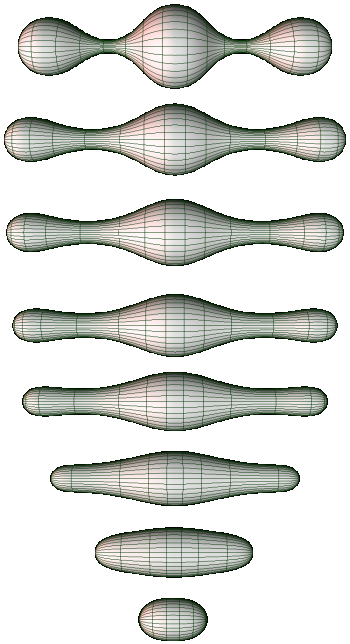
\includegraphics[width=13cm]{ricci-flow.png}
    %     \caption{Ricci flow visualization (Rubinstein, 2005)}
    %     % \label{fig:my_label}
    % \end{figure}

    
    
    
% \section{Exploratory }
    % Recent research in ML, Neuroscience, and Physics strengthens this direction of research; including the GLOM system for representing part-whole hierarchies in neural networks (Hinton 2021), similar part-whole investigations of biological neural trajectories using geometric analysis (Russo et al, 2020), as well as demonstrations of soliton generation from Bose-Einstein condensate. Examining pure mathematics research in ergodic theory and hyperbolic dynamics on moduli spaces enforces the ergodic free-energy minimizing model described in previous notebooks. An encoding mechanism using the cobordism property of the Yang-mills moduli space is also considered.
    
    
    % \subsection{Part-Whole Hierarchies}
    % In Artificial Neural Networks (Hinton 2021): \url{https://arxiv.org/abs/2102.12627}.
    
    % In the brain, using geometric analysis (Russo et al, 2020):
    
    % \url{https://www.sciencedirect.com/science/article/abs/pii/S0896627320303664}.
    
    % \url{https://www.sciencedirect.com/science/article/abs/pii/S0092867420312289}
    
    % \subsection{Cobordism}
    % Moduli of Yang–Mills connections have been most studied when the dimension of the base manifold $X$ is four. Here the Yang–Mills equations admit a simplification from a second-order PDE to a first-order PDE, the anti-self-duality equations. 
    % Additionally, these manifolds demonstrate a cobordism property where in specific circumstances (when the intersection form is definite) the moduli space of ASD instantons on a smooth, compact, oriented, simply-connected four-manifold $X$ gives a cobordism between a copy of the manifold itself, and a disjoint union of copies of the complex projective plane ${\displaystyle \mathbb {CP} ^{2}}$. This might provide a natural and gauge invariant method of dimensionality reduction to be applied to the hierarchical encoding and decoding of an upper bounding layer.
        

% \newpage
\textit{Work in progress}
\newpage

% \subsubsection{Self-Organized Criticality}
%     Condensation of instantons (and noise-induced anti-instantons) are believed to be the explanation of the noise-induced chaotic phase known as self-organized criticality.

%     \url{https://arxiv.org/pdf/1102.1791.pdf}
    
%     parameterizing SOC by gaussian noise may be useful in drawing statistical comparisons between biological neural networks (via connectome harmonic analysis and the Abelian sandpile group) and quantum phenomena.

\begin{comment}
\section{Exploratory }
    \subsection{Cobordism}
        Moduli of Yang–Mills connections have been most studied when the dimension of the base manifold $X$ is four. Here the Yang–Mills equations admit a simplification from a second-order PDE to a first-order PDE, the anti-self-duality equations. 
        Additionally, these manifolds demonstrate a cobordism property where in specific circumstances (when the intersection form is definite) the moduli space of ASD instantons on a smooth, compact, oriented, simply-connected four-manifold $X$ gives a cobordism between a copy of the manifold itself, and a disjoint union of copies of the complex projective plane ${\displaystyle \mathbb {CP} ^{2}}$. This might provide a natural and gauge invariant method of dimensionality reduction to be applied to the hierarchical encoding and decoding of an upper bounding layer.
        
    \subsection{Part-whole Hierarchies}
    \subsubsection{In Artificial Neural Networks (GLOM)}
    
    \url{https://arxiv.org/abs/2102.12627}
    
    \subsubsection{In the Brain}
    \url{https://www.simonsfoundation.org/2021/04/07/geometrical-thinking-offers-a-window-into-computation/}
    
    \url{https://www.sciencedirect.com/science/article/abs/pii/S0092867420312289}
    
    \url{https://www.sciencedirect.com/science/article/abs/pii/S0896627320303664}
    
    
% \section{Ideas and Experiments}
%     does cobordism of moduli enable encoding via dimensionality reduction heirarchy. Symmetry/Guage equivarient hierarchical auto encoder. Symmetry of time to symmetry of space in particle and boson, next is approximate/broken symmetry in hierarchy (and lateral).  
    
%     If the brain indeed has ergodic dynamics imitable through a bernoulli scheme, then this architecture and 

%     The Abelian sandpile group describes a manifold that is able to be parameterized by its points of self-localized criticality.   The sandpile model is a rudimentary cellular automaton defined on a rectangular domain of the standard square lattice

%     Conversely, the computation of n a (lattice) gauge theory with unknown parameters can be done using machine learning techniques

    % on which inference can be performed using natural gradient descent where minima are
% \section{}
%     % https://arxiv.org/pdf/1705.05582.pdf
%     Machine Learning of Explicit Order Parameters: From the Ising Model to SU(2) Lattice Gauge Theory

% \subsection{Harmonic Model Interpretation}

% \subsubsection*{Connectome-Specific Harmonics}

% \subsubsection*{Abelian Sandpile Self-Local Criticality}
%     % https://www.pnas.org/content/116/8/2821
    
%     The Abelian sandpile model offers an interesting experimental opportunity for a manifold to be parameterized by its self-localized criticality. 
    
%     The sandpile model is a cellular automaton defined on a rectangular domain of the standard square lattice




% \subsection{Dimensionality Reduction}
% \subsubsection*{Cobordism}

\subsection{Dynamics}

\subsubsection{Ergodic theory on Moduli Spaces}

\url{https://annals.math.princeton.edu/articles/13160}

 Hyperbolic Dynamics

\url{http://scholarpedia.org/article/Hyperbolic_dynamics#Uniform_hyperbolicity}


\subsubsection{Connectome-specific Harmonic Waves}

\url{https://www.pnas.org/content/116/8/2821}

% See: The Hyperbolic Geometry of DMT Experiences

\subsubsection{Harmonic Dynamics of the Abelian Sandpile}
\url{https://www.pnas.org/content/116/8/2821}

%     Through the process of unfolding, i.e., passing from a polygonal billiard table to a Riemann manifold equipped with a holomorphic 1-form, a billiard trajectory which reflects off the sides of the table unfolds into a straight line or geodesic on the manifold. We define the symmetry group$ SL(X, \omega)$ associated to any translation surface. We extend the notions of ergodically optimal and topologically optimal to general translation surfaces. Finally, we introduce the notion of a lattice surface and compare it to an ergodically optimal surface.

\subsection{Physics}
    \subsubsection{Condesate of Instantons as Variational EBM}
    
    Energies can be thought of as being \textit{unnormalized negative log probabilities}. That is, we may use the Gibbs-Boltzmann distribution to convert an energy function to its equivalent probabilistic representation after normalization, i.e. $P(y \mid x)$. Recall, \textit{marginalisation} is a method that sums over the possible values of one variable to determine the marginal contribution of another. $P(y \mid x)$ is just an application of the Gibbs-Boltzmann formula with latent variables $z$ being marginalized implicitly through integration, i.e. $P(y \mid x) = \int_z P(y,z | x)$. Then,
    \begin{align*}
        P(y \mid x) &= \frac{ \int_z \exp(-\beta E(x,y,z)) }{ \int_y \int_z \exp(-\beta E(x, y, z))} \\
        % &= \frac{
        %     \exp \bigg [  -\beta (-\frac{1}{\beta} \log  \int_z \exp(-\beta E(x,y,z)) ) \bigg ]
        % }{
        %     \int_y \exp \bigg [  -\beta (-\frac{1}{\beta} \log  \int_z \exp(-\beta E(x,y,z)) ) \bigg ]
        % }
    \end{align*}
    The derivation introduces a $\beta$ term which is the inverse of temperature $T$, so as $\beta \rightarrow \infty$ the temperature goes to zero. $\beta$ is a positive constant that needs to be calibrated to fit the model. A larger $\beta$ value produces a more fluctuate model while a smaller $\beta$ gives a smoother model. When $\beta \rightarrow \infty$, we see that $\check{y} = \text{argmin}_{y} E(x,y)$. So we can redefine our energy function as an equivalent function using $F_\beta$,
    \begin{align*}
        F_{\infty} (x,y) &= \text{argmin}_z E(x,y,z)\\
        F_{\beta} (x,y) &= -\frac{1}{\beta} \log \int_z \exp(-\beta E(x,y,z)).
    \end{align*}
    
    In physics, $F_\beta$ is known as the free energy and $E$ is the energy. If we have a latent variable model and want to eliminate the latent variable $z$ in a probabilistically correct way, we just need to redefine the energy function in terms of $F_\beta$,
    \[
        P(y \mid x) = \frac{ \exp(-\beta F_\beta(x,y,z)) }{ \int_y \exp(-\beta F_\beta(x, y, z))}. \\
    \]
    
    \subsubsection{Self-Organized Criticality}
    In physics, instantons are particularly important because the condensation of instantons (and noise-induced anti-instantons) is believed to be the explanation of the noise-induced chaotic phase known as self-organized criticality.

    \subsubsection{Bose-Einstein Condesate and Solitons}
    
    Observation of Magnetic Solitons in a Bose-Einstein Condensate
    \url{https://physics.aps.org/articles/v13/s90}
    
    % https://www.researchgate.net/publication/51360828_Generating_Solitons_by_Phase_Engineering_of_a_Bose-Einstein_Condensate
    
    
    Spatial phase distributions were optically imprinted onto a Bose-Einstein condensate (BEC) of atoms and was shown to create solitons.
    
    \url{https://science.sciencemag.org/content/287/5450/97}
    
    \begin{multicols}{2}
    \noindent
    \begin{align*}
        {\displaystyle \,T_{\rm {c}}} \,  &\text{is the critical temperature,}\\
        \displaystyle \,n \, 	 &\text{ the particle density,}\\
        {\displaystyle \,m}	\, &\text{the mass per boson,}\\
        {\displaystyle \hbar } \, 	&\text{the reduced Planck constant,}\\
        {\displaystyle \,k_{\rm {B}}}\, 	&\text{the Boltzmann constant and}\\
        {\displaystyle \,\zeta }\, 	&\text{the Riemann zeta function;}
    \end{align*}
    \begin{align*}
        {\displaystyle T_{\rm {c}}=\left({\frac {n}{\zeta (3/2)}}\right)^{2/3}{\frac {2\pi \hbar ^{2}}{mk_{\rm {B}}}}}
    \end{align*}
    \end{multicols}
    \subsubsection*{Superliminal Solitons from Hyperbolic Shift Vectors}
    \url{https://arxiv.org/abs/2006.07125}




% \subsection*{Hyperbolic Dynamics}

% \subsubsection{Conformal Invariance}

    \subsection{Geometric Unity and Anthropic Principle}
    
    \url{https://geometricunity.nyc3.digitaloceanspaces.com/Geometric_Unity-Draft-April-1st-2021.pdf}
    
\end{comment} 

\section*{References}

\small

[1] Gao, Tingran. "The diffusion geometry of fibre bundles: Horizontal diffusion maps." Applied and Computational Harmonic Analysis 50 (2021): 147-215.
% https://arxiv.org/pdf/1602.02330.pdf

[2] Eckhard Meinrenken, "Principal bundles and connections", Lecture Notes. 
% http://www.math.toronto.edu/mein/teaching/moduli.pdf

[3] Tao, T. "What is a gauge?" (2008) https://terrytao.wordpress.com/2008/09/27/what-is-a-gauge/
% https://terrytao.wordpress.com/2008/09/27/what-is-a-gauge/

[4] Wetzel, Sebastian J., and Manuel Scherzer. "Machine learning of explicit order parameters: From the Ising model to SU (2) lattice gauge theory." Physical Review B 96.18 (2017): 184410.
% https://arxiv.org/pdf/1705.05582.pdf


[5] Du, Yilun, and Igor Mordatch. "Implicit generation and generalization in energy-based models." arXiv preprint arXiv:1903.08689 (2019).
% https://arxiv.org/abs/1903.08689

[6] Blei, David M., Alp Kucukelbir, and Jon D. McAuliffe. "Variational inference: A review for statisticians." Journal of the American statistical Association 112.518 (2017): 859-877.

% [3] Paul, Arnab, and Suresh Venkatasubramanian. "Why does deep learning work?-a perspective from group theory." arXiv preprint arXiv:1412.6621 (2014).
% https://arxiv.org/pdf/1412.6621.pdf

[7] Hinton, Geoffrey. "How to represent part-whole hierarchies in a neural network." arXiv preprint arXiv:2102.12627 (2021).

[8]  Yann LeCun, DS-GA 1008, DEEP LEARNING, NYU CENTER FOR DATA SCIENCE

[9] Russo, Abigail A., et al. "Neural trajectories in the supplementary motor area and motor cortex exhibit distinct geometries, compatible with different classes of computation." Neuron 107.4 (2020): 745-758.

[10] Farolfi, A., et al. "Observation of magnetic solitons in two-component Bose-Einstein condensates." Physical Review Letters 125.3 (2020): 030401.

[11] Denschlag, J., et al. "Generating solitons by phase engineering of a Bose-Einstein condensate." Science 287.5450 (2000): 97-101.

[12] J. Hyam Rubinstein and Robert Sinclair. "Visualizing Ricci Flow of Manifolds of Revolution", Experimental Mathematics v. 14 n. 3, pp. 257–384

% https://ncatlab.org/nlab/show/principal+bundle


% % % % % % % % % % % % % % % % % % % % % % % % % % % % % % % % % % % % 




\begin{comment}
% The gauge theoretic model of neural activity is described using fiber and vector bundles with their respective connections (covariant derivatives). 
    
    % The moduli space of connections can be formulated by quotienting the space of principal connections by its gauge group, generating a gauge equivariant space that is also a smooth and finite dimensional manifold. This can be formalized as a Yang-Mills moduli space or as a moduli space of principal flat connections. 


    % https://papers.nips.cc/paper/2017/file/0ebcc77dc72360d0eb8e9504c78d38bd-Paper.pdf
    
    % This study deals with neural networks in the sense of geometric transformations
    % acting on the coordinate representation of the underlying data manifold which
    % the data is sampled from. It forms part of an attempt to construct a formalized
    % general theory of neural networks in the setting of Riemannian geometry. From
    % this perspective, the following theoretical results are developed and proven for
    % feedforward networks. First it is shown that residual neural networks are -
    % nite dierence approximations to dynamical systems of rst order dierential
    % equations, as opposed to ordinary networks that are static. This implies that the
    % network is learning systems of dierential equations governing the coordinate
    % transformations that represent the data. Second it is shown that a closed form
    % solution of the metric tensor on the underlying data manifold can be found by
    % backpropagating the coordinate representations learned by the neural network
    % itself. This is formulated in a formal abstract sense as a sequence of Lie group
    % actions on the metric bre space in the principal and associated bundles on the
    % data manifold


    
    % introduce Ergodic justifactions:
    % - recursive neuron structure uses joint divergence 
    % Applications of this manifold in machine-learning may prove useful in the task of meta-learning, i.e. classification of inputs into subtasks and subnetworks, as well as in pre-training covariance. Lastly, examining mathematical research in ergodic dynamics of Moduli spaces allows the ergodic free-energy model described in previous works to be developed further.


    % Theorem 1 ([Her60],[Bes07, Theorem 9.3]). Let pi : E → M be a Riemannian submersion (c.f. [Bes07, Definition 9.8]). If E is a complete, then pi : E → M is a fibre bundle

    % In a nutshell, Hermann explicitly constructed local trivializations around each x ∈ M, by connecting points on the fibre pi −1 (x) to points on any neighboring fibre pi −1 (y) by horizontally lifting the geodesic on M that connects x to y. Here the horizontal lifting is made possible by the Riemannian structure on E, which canonically splits the tangent bundle of E into the direct sum of a horizontal and vertical subbundles. As pointed out in [Bes07, §9.E], the horizontal subbundle is an Ehresmann connection (see A) on the fibre bundle. The structure group of the fibre bundle can then be determined from the holonomy of the Ehresmann connection; see [Bes07, §9.47] for more details. 
    
    % In other words, a fibre bundle can be defined equivalently by a smooth submersion between the total and base manifold (with appropriate completeness assumptions), a Riemannian structure on the base manifold, and an Ehresmann connection. We close the discussion in this section by emphasizing that, though it might appear that our fibre bundle framework “discards” the notion of structure groups compared with the fibre bundle formulation pioneered in [SW12, SW16], structure groups indeed are specified, just in an indirect manner.
\end{comment}



\begin{comment}
\section{Definitions}
    % - Kernel space
    % - feature space

    % Manifolds appear frequently in macine learning and statistical learning; in the form of cost functions, divergences, kernel spaces, feature space

    Input Space ($X$): It is the original space that the signal inhabits. Most signals of interest are compactly supported bounded real functions over a vector space $X$. The function space is denoted by $C^0(X,\mathbb R) = {\phi | \phi : X \rightarrow \mathbb R}$. We define Intrinsic space as: $S = X \times \mathbb R$. Every $\phi \in C^0(X, \mathbb R)$ is a subset of $S$. A neural network maps a point in $C^0(X, \mathbb R)$ to another point in $C^0(X,\mathbb R)$; Inside $S$, this induces a deformation between subsets.
    
    Figure: A subset of the intrinsic space is called a figure, i.e., $f \subseteq S$. Note that a point $\phi \in C^0(X,\mathbb R)$ is actually a figure over $S$.
    
    Moduli space of Figures: One can imagine a space that parametrizes various figures over $S$. We denote this by $F(S)$ and call the moduli space of figures. Each point in $F(S)$ corresponds to a figure over $S$. A group $G$ that acts on $S$, consistently extends over $F(S)$, i.e., for $g \in G, f \in S$, we get another figure $g(f) = f' \in F(S)$.
    
    
    At its root, lies the principle of layer-wise pre-training for the identity function. In particular, we show that this succinct step, as an algorithmic principle, is quite powerful. The principle stays the same across layers; hence every layer only learns the simplest possible objects from its own input space. Yet, a simple objects at a deeper layer can represent a complex object at the input space. This construction is recursive over layers, so one can envision a neural net building representations of moduli spaces over moduli spaces, hierarchically, one after another. These moduli-spaces are determined by the underlying input-space, and the nature of training. So, doing precise calculations over them, such as defining the space of all automorphisms, or computing volumes over corresponding stabilizer sets, may be very difficult.
    
    \subsection{Kernel machines}
    \subsection{Attention}
    \subsection{Pretraining}
\end{comment}

\begin{comment}
\section{Appendix}
\subsection{Fiber and vector bundles}
    A \textit{fiber bundle} serves as a useful mathematical object to analyse both the recursive behaviour of artificial and biological neurons and neural networks, as well as their application in information processing and manifold representation. A fiber bundle makes precise the idea of one topological space (called a fiber) being ``parameterized'' by another topological space (called a base). The bundle also comes with a group action on the fiber that represents the different ways the fiber can be viewed as equivalent. Let $F$ be a given manifold. A smooth fiber bundle with standard fiber $F$ is a smooth map $\pi : E \rightarrow B$ from a manifold $E$ (the total space) to a manifold $B$ (the base) with the following property, called local triviality: There exists an open covering $U_\alpha$ of $B$ and difeomorphisms 
    \[
        \phi_\alpha : \pi^{-1}(U_\alpha) \rightarrow U_\alpha  \times F
    \] 
    such that $\hbox{proj}_{U_\alpha}(\phi(x)) = \pi(x)$. Recall, a diffeomorphism is an isomorphism of smooth manifolds, so $\phi$ intertwines $\pi$ with projection to the first factor. We will denote the fibers by $E_b = \pi^{-1}(b)$. Additional structures on $F$ give rise to special types of fiber bundles:
    \begin{itemize}
        \item If $F = V$ is a vector space, one defines a \textit{vector bundle} with standard fiber $V$ to be a fiber bundle $\pi : E \rightarrow B$ where all fibers $\pi^{-1} (b)$ are vector spaces and the local trivializations $\phi_\alpha$ can be chosen to be fiberwise linear. A homomorphism of two vector bundles is a fiber bundle homomorphism that is fiberwise linear. The fibered product of vector bundles $E_1; E_2$ is a vector bundle (also called Whitney sum and denoted $E1 \oplus E2$).
        
        \item Recall, a Lie group is a group that is also a differentiable manifold where points can be multiplied together, they have inverses, and these operations are defined to be smooth (differentiable). If $F = G$ has the structure of a Lie group, one defines a \textit{group bundle}, $\mathcal G \rightarrow B$ with standard fiber $G$ to be a fiber bundle where all fibers carry group structures and the local trivializations can be chosen to be a fiberwise group homomorphisms. A group bundle homomorphism is a fiber bundle homomorphism which is fiberwise a group homomorphism. The fibered product of group bundles is a group bundle. One has natural bundle maps $\mathcal G \times^B \mathcal G \rightarrow \mathcal G$ (fiberwise group multiplication) and $\mathcal G \rightarrow \mathcal G $ (fiberwise inversion). Similarly, one defines algebra bundles, Lie algebra bundle as well as fiberwise linear actions of group or algebra bundles on vector bundle.
        
        \item  A principal $G$-bundle (also called a G-torsor over X) share similar properties to the resulting space of a Cartesian product of a space with a group. They are a fiber bundle $\pi: \mathcal P \rightarrow X$ together with a continuous right action $\mathcal P \times G \rightarrow \mathcal P$ such that $G$ preserves the fibers of $\mathcal P$ (i.e. if $y \in \mathcal P_x$ then $yg \in \mathcal P_x$ for all $g \in G$) and acts freely and transitively (i.e. regularly) on them in such a way that for each $x\in X$ and $y \in \mathcal P_x$, the map $G \rightarrow \mathcal P_x$ sending $g$ to $yg$ is a homeomorphism. In particular each fiber of the bundle is homeomorphic to the group $G$ itself. One can also define principal $G$-bundles in the category of smooth manifolds. Here $\pi : \mathcal P \rightarrow X$ is required to be a smooth map between smooth manifolds, $G$ is required to be a Lie group, and the corresponding action on $\mathcal P$ should be smooth. 
    \end{itemize}

 
\subsection{Connections}
    The notion of a \textit{connection} defines the idea of transporting data along a curve or family of curves in a parallel and consistent manner. A \textit{covariant derivative} is a linear differential operator which takes the directional derivative of a section of a vector bundle in a covariant manner. It also allows one to formulate a notion of a parallel section of a bundle in the direction of a vector: a \textit{section} $s$ is parallel along a vector $X$ if $\nabla _{X}s=0$. An \textit{Ehresmann connection} is a connection in a fibre bundle or a principal bundle made by specifying the allowed directions of motion of the field. Specifically, it singles out a vector subspace of each tangent space to the total space of the fiber bundle, called the horizontal space. A section $s$ is then horizontal (i.e., parallel) in the direction $X$ if $\rm {d}s(X)$ lies in a horizontal space.

    For any fiber bundle $\pi : E \rightarrow B$ the tangent bundle $T E$ of the total space has a distinguished subbundle, the vertical bundle $V E \hookrightarrow T E$. The fiber $V_xE$ for $\pi(x) = b$ is the image of $T_x(F_b)$ under the natural inclusion $T F_b \hookrightarrow T E$. An Ehresmann connection on $E$ is the choice of a complementary horizontal subbundle $HE$ such that $T E = V E \oplus HE$. Equivalently, a connection is a bundle projection $T E \rightarrow V E$ which is left-inverse to the inclusion $V E \rightarrow T E$; one defines $HE$ as the kernel of this projection. 
    
    The Ehresmann connection has the immediate benefit of being definable on a much broader class of structures than vector bundles and is well-defined on a general fiber bundle. Many of the features of the covariant derivative still remain: parallel transport, curvature, and holonomy. With the classical covariant derivatives, covariance is an a posteriori feature of the derivative. However, for an Ehresmann connection, it is possible to impose a generalized covariance principle from the beginning by introducing a Lie group acting on the fibers of the fiber bundle. The appropriate condition is to require that the horizontal spaces be equivariant with respect to the group action.

    If the standard object $F$ has additional structure, one is interested in connections such that parallel transport preserves that structure. For example, if $E$ is a vector bundle, each parallel transport operation, $\Pi^\gamma$, should be a linear map, and for group bundles it should be a fiberwise group homomorphism, and so on.
    An important special case of Ehresmann connections are principal connections on principal bundles, which are required to be equivariant in the principal Lie group action.   A principal connection on a fiber bundle is an equivariant Lie algebra valued 1-form $\theta \in \Gamma^1 (\mathcal P, \mathfrak g)^G$ such that $\iota(\xi_{\mathcal P})\theta = \xi$ (where $\iota$ is an inclusion embedding) for all $\xi \in \mathfrak g$, the Lie algebra.  
    
    The space of principal connections will be denoted $\mathcal A(P)$. The space $\mathcal A(P)$  has a natural affine structure, with underlying vector space the space $\Gamma^1 (B, \mathfrak g( \mathcal P))$ of 1-forms on $B$ with values in the adjoint bundle.



\subsection{Gauges}
    
    A gauge can be thought of as a coordinate system that varies depending on one’s location with respect to some base space or parameter space. A gauge transform is a change of coordinates applied to each such location, and a gauge theory is a model for some physical or mathematical system to which gauge transforms can be applied and is typically gauge invariant, in that all physically meaningful quantities are left unchanged or transform naturally under gauge. A principal bundle automorphism is a $G$-equivariant diffeomorphism $\phi : \mathcal P \rightarrow \mathcal P$ taking fibers to fibers. The group of principal bundle automorphisms will be denoted $\hbox{Aut}( \mathcal P)$. 
    
    The space of "coordinate systems" is (non-canonically) identifiable with the isomorphism group $\hbox{Isom}(G)$ of template $G$.  This isomorphism group is called the structure group or gauge group of the class of geometric objects. The gauge group $\hbox{Gau}( \mathcal P) \subseteq \hbox{Aut}(\mathcal P)$ consists of automorphisms $ \phi : \mathcal P \rightarrow \mathcal P$ inducing the identity map on the base $B$. That is, $\hbox{Gau}( \mathcal P)$ is defned by an \textit{exact sequence} of groups
    \[
        1 \longrightarrow \hbox{Gau}( \mathcal P) \longrightarrow \hbox{Aut}( \mathcal P) \longrightarrow \hbox{Diff} B)
    \]
    Let $\theta$ be a principal connection on $\pi : \mathcal P \rightarrow B$. For any path $\gamma : [t_0, t_1] \rightarrow B$, let 
    \[
        \Pi^\theta_\gamma : P_{\gamma(t_0)} \rightarrow P_{(t_1)} 
    \]
    denote parallel transport with respect to $\theta$. For all $\phi \in \hbox{Gau}(\mathcal P)$,
    \[
        \Pi_{\gamma}^{\phi,\theta} = \phi(\gamma(t_1)) \circ  \Pi_{\gamma}^{\theta} \circ  \phi(\gamma(t_0))^{-1}
    \]
    The group of automorphisms $\hbox{Aut}( \mathcal P)$ acts on the space $\mathcal A( \mathcal P)$ of principal connections by pull-back by the inverse. This can be understood as the gauge transformations of connections. We can interpret $\mathcal A( \mathcal P)$ as an infinite dimensional manifold, equipped with an action of an infinite-dimensional Lie Group. 
    % The generating vector field for the action of the bundle section $\zeta$ on $\mathcal A( \mathcal P)$ is given by the covariant differential.
    

    % For the action of the subgroup $\hbox{Gau}( \mathcal P)$, there is an alternative formula for this action.

\section{Moduli Spaces}
    The quotient space of the space of principal connections and the Gauge  $\mathcal A(P) / \hbox{Gau}(P)$ is called the moduli space of connections. It is still infnite-dimensional. To obtain a finite dimensional moduli spaces, one has to impose additional gauge-invariant constraints on $\theta$: e.g. that it is a flat connection, or more generally a Yang-Mills connection. Suppose $\pi : \mathcal P \rightarrow B$ is a principal $G$-bundle over a compact, oriented, Riemannian manifold $B$. The inner product on $T B$ gives rise to an inner product on $T M$ and on all $ \wedge^k T^*M$. Taking the inner product of the differential form, followed by integration over $B$ with respect to the Riemannian volume form, defines an inner product on $\Omega^* (B)$. In terms of the Hodge star operator, 
    \[
        \langle \alpha, \beta \rangle = \int_B \alpha \wedge  * \beta
    \]
    Let $|| \cdot ||$ be the norm corresponding to $\langle \cdot, \cdot \rangle$. The Yang-Mills functional on $\mathcal A(\mathcal P)$ is the functional 
    \[
        \hbox{YM}(\theta) = ||F ||^2 = \int_B (F^\theta, * F^\theta)
    \]
    The Yang-Mills functional is invariant under the action of the gauge group, i.e. $YM(\theta) = YM(\phi,\theta)$, hence all its critical points (called Yang-Mills connections) are invariant as well. A connection $\theta$ is a critical point of the Yang-Mills functional if and only if it satisfies the Yang-Mills equation, $d^\theta * F^\theta = 0$. The quotient of the space of Yang-Mills connections by the action of the gauge group is called the Yang-Mills moduli space. In this context, the term ``moduli'' is used synonymously with ``parameter''. 
    
    
    Moduli of Yang–Mills connections have been most studied when the dimension of the base manifold X is four. Here the Yang–Mills equations admit a simplification from a second-order PDE to a first-order PDE, known as the anti-self-duality equations. The Yang-Mills equations depend upon the Riemannian metric on $B$ only via the star operator on $\Gamma^2 (B)$. The case $\dim B = 4$ is special in that it takes $\Gamma^2 (B)$ to itself, since $4 - 2 = 2$. We mentioned already that in this case the Yang-Mills equations are conformally invariant: Multiplying the metric by a positive function does not change the star operator in middle dimension, hence does not change the Yang-Mills equations. A special type of Yang-Mills connections in $4$ dimensions are those satisfying one of the equations 
    \[
        *F^\theta = F^\theta \text{\ \ or \ \  }  *F^\theta = - F^\theta 
    \]
    (self-duality and anti-self-duality respectively) because for such connections, the Yang-Mills equations are a consequence of the Bianchy identity $d^\theta F^\theta = 0$. A change of orientation of $B$ changes the sign of the  operator, and therefore exchanges the notion of duality and anti-self duality. For certain principal bundles ($\theta$ is a multiple of the second Chern number), ASD connections give the absolute minimum of the Yang-Mills functional.
    
    % Anti-self dual connections over S4 are also called instantons.
    
    % The moduli space for anti-self dual YM-connections for G = SU(2) is the starting point for Donaldson theory of 4-manifolds. As realized by Donaldson, they contain information not only about the topology but also the differentiable structure of 4-manifolds.
    
\end{comment}    

\end{document}
